%!TEX root = ../ArticleCalib_main.tex

%%%%%%%%%%%%% FIGURE 4 : SNR / TAU OPTIMAL SEGMENTATION


\begin{figure}[htbp]
\begin{center}
\captionsetup[subfigure]{position=top, labelfont=bf, textfont=normalfont, singlelinecheck=off, justification=raggedright }

\subfloat[]{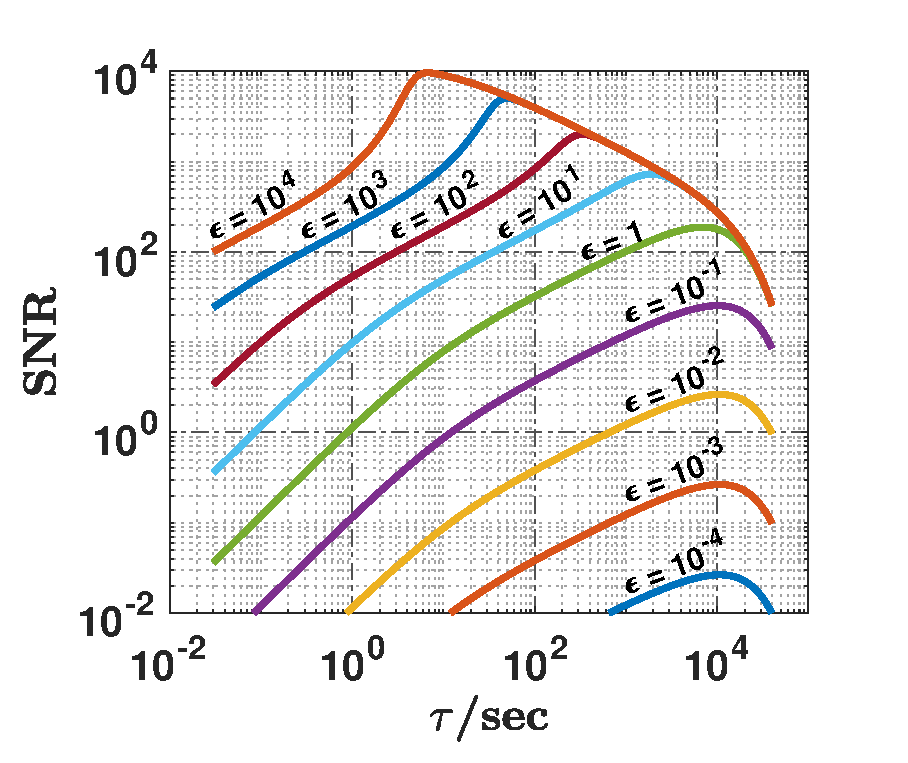
\includegraphics[width=0.4\linewidth]{fig4_model_segmentation/fig4A_SNRtau.eps}\label{fig:SNRTau:A}}  \qquad
\subfloat[]{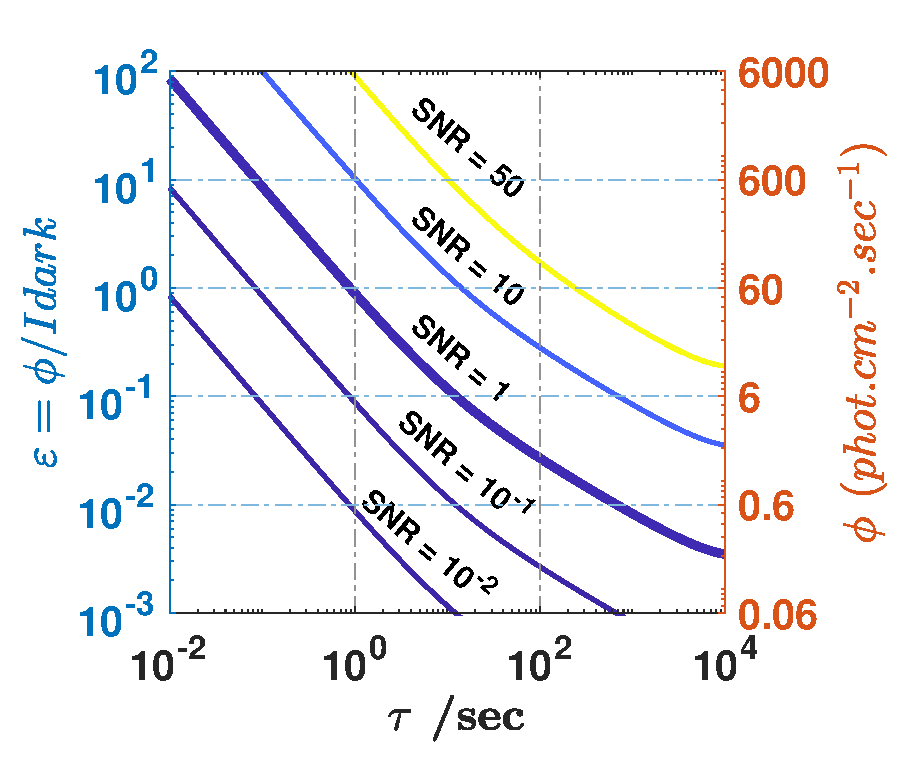
\includegraphics[width=0.4\linewidth]{fig4_model_segmentation/fig4B_SNRcontour.eps}\label{fig:SNRTau:B}}  \\

\subfloat[]{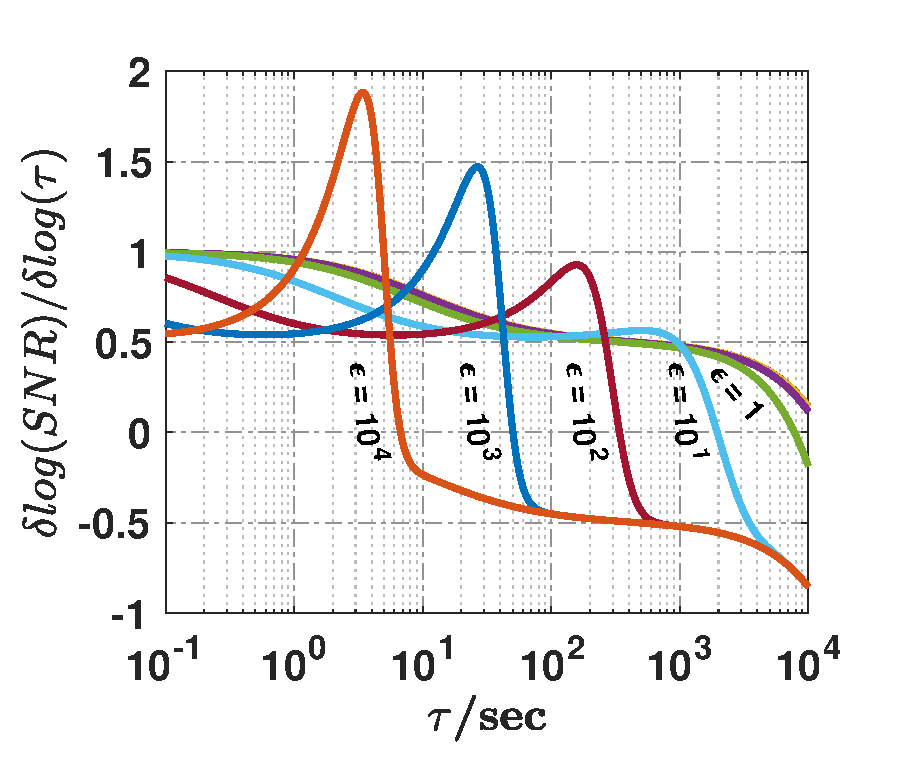
\includegraphics[width=0.4\linewidth]{fig4_model_segmentation/fig4C_derivelogSNRTau.eps}\label{fig:SNRTau:C}} \qquad
\subfloat[]{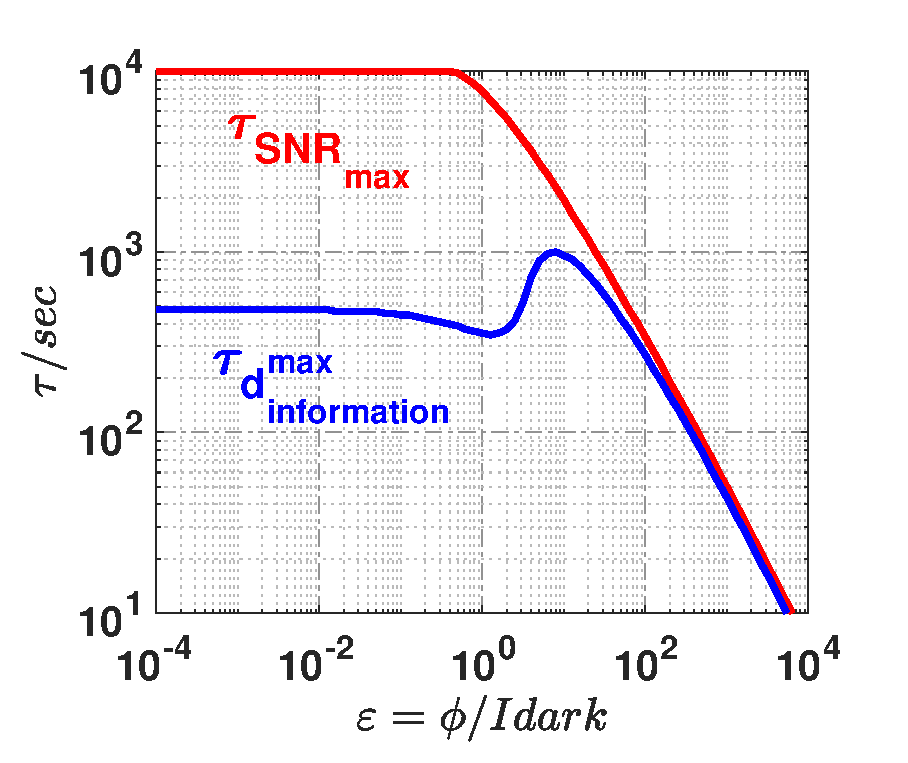
\includegraphics[width=0.4\linewidth]{fig4_model_segmentation/fig4D_SNRtaudensitemax_snrmax.eps}\label{fig:SNRTau:D}}. \\


\caption{{\bf SNR simulation.} The SNR simulation is represented for different fluxes $\phi$ expressed as a fraction $\epsilon$ of the dark current Id. The x axes is extended to $10^5$ seconds to show the effect of the saturation on the SNR in photon counting mode \subref{fig:SNRTau:A}. Figure  \subref{fig:SNRTau:B} shows the corresponding SNR contour plot.
{\bf What is the optimal time of exposure.}  Figure \subref{fig:SNRTau:C} shows the logarithmic derivative of the SNR ($\delta logSNR/\delta log\tau$) for different fluxes. The time of maximal information density ($\tau_{d_{info}^{max}}$) is such as  $\delta logSNR/\delta log\tau = 0,5$  \subref{fig:SNRTau:D}. The time of maximal SNR  ($\tau_{SNR^{max}}$) is comparatively represented. }
\label{fig:SNRTau}
\end{center}
\end{figure}
%%%%%%%%%%%%%%%%%%%


